\section{A Series of Tubes}

\section{Tool for Tube Design}

We created a tool which novice designers can use to create tube-powered interfaces in arbitrary 3D models.  This tool allows users to brush over the surface of their model to either select exterior connection points of their tubes (see Figure \ref{fig:tool-process-interior}) or to author the tubes' interior paths (see Figure \ref{fig:tool-process-exterior}).  Once the user's selections are made, our tool creates an initial shortest-path routing using A* to estimate the routed distance between points.  This routing is used to create a rod; we run physics-based simulation steps on the rod to minimize its bending energy (and thereby minimize the bend radius of the tubes).  The resultant routing is subtracted from the user's mesh.  The modified mesh can then be 3D printed.

\subsection{Exterior Connection Points}

\begin{figure}[h!]
\centering
    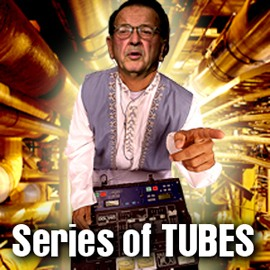
\includegraphics[width=3.4in]{figures/series-of-tubes.jpg}
\caption{This figure has several sub-figures.  a) shows a model with exterior connection points brushed.  b) shows initial routing with A*.  c) shows our physics-based, energy-minimizing rod/tube, d) shows the printed object with the tube (with something in it, copper paint presumably)}
\label{fig:tool-process-exterior}
\end{figure}

\subsubsection{Routing}

Focus on shape of points and location of points.

\subsubsection{Routing}

Our basic first-pass routing algorithm uses the A* routing algorithm \cite{Hart-Astar}.  The path cost in our implementation is based only on shortest distance between the starting and ending points, without weighting for distance from the surface.

Physical Simulation : 

How does it actually work?

Bend Minimization

Collision detection

\subsection{Designing Interior Paths}

\begin{figure}[h!]
\centering
    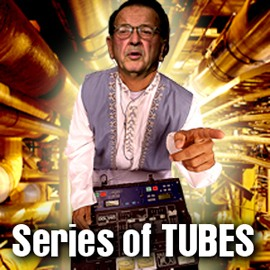
\includegraphics[width=3.4in]{figures/series-of-tubes.jpg}
\caption{This figure has several sub-figures.  a) shows a model with path shape and exterior connection point(s) brushed.  b) highlights the points which can't be tubed as drawn (if they are not connected, too tight, etc.).  c) shows our physics-based, energy-minimizing rod/tube and any path-smoothing that we do, d) shows the printed object with the tube (with something in it, EL wire presumably)}
\label{fig:tool-process-interior}
\end{figure}

take into account bend radius of desired material - no need, we just do the minimum-bending path

Our problem here is a relaxed version of the Chinese Postman Problem$^{[\valkyrie{citation needed}]}$ in which we wish to traverse all edges of the graph described in the user's input (as the edges of the graph are the lines the user wishes to have lit) with a single circuit.  It is a relaxation in that we allow the creation of non-existing paths: if components are disconnected (e.g., a user wishes to spell ``UIST" in neon lights), we must create edges that connect them; additionally we can create edges to connect odd-degree vertices rather than simply retracing existing edges.  In the final design, all created edges will be shielded by dark material so the inserted medium is not visible.

We want a semi-Eulerian graph (i.e., we want a graph in which every vertex but two have even degree) so that the desired medium can be inserted, traverse every edge, and exit the graph at a different vertex.

Let $G=(V,E_0)$ s.t. $\forall e \in E_0, weight(e)=0, start \in V $ the start point $end \in V$ the end point.  Let $e_{temp} = (start, end)$, $E' = e_{temp} \cup E$.

We need to connect disconnected subgraphs in $G$.  Let $G_{dis} = \{G_1, G_2, ... G_n\} \in G$ s.t. $\cup{\{G_i \in G_{dis}\}} = G$ and $G_i \cap G_j  = \{ \} \forall G_i, G_j \in G_{dis}, i\neq j$ be disconnected subgraphs in G.  Create $E_{conn} = \{e = (u, v), u \in G_i, v \in G_j, i \neq j, weight(e) = distance(u, v)\}$ be a set of edges.  Sort $E_{conn}$ s.t. $E_{conn} = \{e_1, e_2, ... e_n\}, weight(e_1) \leq weight(e_2) \leq \ldots \leq weight(e_n)$.  Let $E_{conn-min} = \{ \}$.

Beginning with $e_1$, add the first edge $e_i \in E_{conn}$ to $E_{conn-min}$.  Then let $E_{dupe} = \{ e = (u, v) \in E_{conn}$ s.t. $u$  is reachable from $v$ along edges $E' \cup E_{conn-min}$.  Let $E_{conn} = E_{conn} \setminus E_{dupe}$.  Repeat until $E_{conn} = \{ \}$.  Let $E' = E' \cup E_{conn-min}$.

At this stage, we want an Eulerian graph: i.e., we need every vertex to be of even degree.  Let $V_{odd} = \{ v \in V s.t. degree(v) \% 2 = 1 \}$.  Create $E_{circuit} = V_{odd} \times V_{odd}$, s.t. $\forall e=(u,v) \in E_{circuit}, weight(e) = distance(u, v)$.  Find minimum matching $E_{circuit-min} \subseteq E_{circuit}$.  Let $E' = (E\setminus e_{temp}) \cup E_{circuit-min}$.

\begin{theorem}
 $G' = (V, E')$ is a connected, semi-Eulerian graph for which $E \subseteq E'$.
\end{theorem}
\begin{proof}
$E \subseteq E'$ : we never remove edges from $E$ in our algorithm.  $\therefore E \subseteq E'$.

$G' = (V, E')$ is connected : if $G'$ is not connected, $\exists G_i = (V_i, E_i) \subset G', u \in V_i, v\in V \setminus V_i$ s.t. $u$ is not reachable from $v$.  $G_i \not\in G_{dis}$, because we create edges connecting $G_j, G_k \forall G_j, G_k \in G_{dis}$ and only remove an edge $e_{dupe} = (u, v)$ from $E_{conn}$ once we determine that $u$ is reachable from $v$ along edges $E' \cup E_{conn-min}$.  $\therefore G_i \not\in G_{dis}$.  This implies that $G_i$ was not initially disconnected from $G$, because by definition $G_{dis}$ is the set of all disconnected subgraphs of $G$.  We cannot have disconnected $G_i$ from $G$ because $E \subseteq E'$.  Thus, a contradiction.  $\therefore G' = (V, E')$ is connected.

$G' = (V, E')$ is semi-Eulerian : Each edge $e$ in our minimum weight matching connects a unique pair of vertices $v_i, v_j \in V_{odd}$ by the definition of minimum weight matching.  Each edge $e = (v_i, v_j) \in E_{circuit-min}$ adds one to the degree of $v_i$ and $v_j$, causing them to be of even degree. $|V_{odd}| \% 2 = 0$ by the handshake lemma, $\therefore$ all edges can be paired.  When we remove $e_{temp} = (start, end)$ from $E'$, we cause those vertices, which were of even degree by the above process, to be of odd degree.  Thus, all vertices except $start$ and $end$ (which are of odd degree) are of even degree.  $\therefore G'$ is semi-Eulerian.
\end{proof}

\subsection{Mesh Modification}

How we actually cut stuff and make tubes happen.

\subsection{Fabrication Techniques}

\subsubsection{Printing} - different strategies with Objet (all print-in-place) and Makerbot (may need to add things like balloons afterwards).  Ryan just got flexible material, we should see how stretchy it is...!  We could also consider assembleable things that are easier to create using parts that clip together... probably out of scope.

\subsubsection{Hand Tools} - post-fabrication modification is possible using hand tools.  We can mark the surface to show where conduits are and how deep.  I can also use this to test things before spending time printing them using a big ol' block o' plastic.